% ------------------------------------------------------------------------
% ------------------------------------------------------------------------
% abnTeX2: Modelo de Trabalho Academico (tese de doutorado, dissertacao de
% mestrado e trabalhos monograficos em geral) em conformidade com 
% ABNT NBR 14724:2011: Informacao e documentacao - Trabalhos academicos -
% Apresentacao
% ------------------------------------------------------------------------
% ------------------------------------------------------------------------

\documentclass[
	% -- opções da classe memoir --
	12pt,				% tamanho da fonte
	openright,			% capítulos começam em pág ímpar (insere página vazia caso preciso)
	oneside,
	%twoside,			% para impressão em verso e anverso. Oposto a oneside
	a4paper,			% tamanho do papel. 
	% -- opções da classe abntex2 --
	%chapter=TITLE,		% títulos de capítulos convertidos em letras maiúsculas
	%section=TITLE,		% títulos de seções convertidos em letras maiúsculas
	%subsection=TITLE,	% títulos de subseções convertidos em letras maiúsculas
	%subsubsection=TITLE,% títulos de subsubseções convertidos em letras maiúsculas
	% -- opções do pacote babel --
	english,			% idioma adicional para hifenização
	francais,			% idioma adicional para hifenização
	spanish,			% idioma adicional para hifenização
	brazil				% o último idioma é o principal do documento
	]{abntex2}

% ---
% Pacotes básicos 
% ---
\usepackage{lmodern}			% Usa a fonte Latin Modern
\usepackage[T1]{fontenc}		% Selecao de codigos de fonte.
\usepackage[utf8]{inputenc}		% Codificacao do documento (conversão automática dos acentos)
\usepackage{lastpage}			% Usado pela Ficha catalográfica
\usepackage{indentfirst}		% Indenta o primeiro parágrafo de cada seção.
\usepackage{color}				% Controle das cores
\usepackage{graphicx}			% Inclusão de gráficos
\usepackage{microtype} 			% para melhorias de justificação

% ---
% Pacotes de citações
% ---
\usepackage[brazilian,hyperpageref]{backref}	% Paginas com as citações na bibl
\usepackage[alf]{abntex2cite}					% Citações padrão ABNT

% ---
% Pacotes gráficos
% ---
\usepackage{graphicx}
\usepackage{tikz}
\usetikzlibrary{shapes,arrows}

% --- 
% CONFIGURAÇÕES DE PACOTES
% --- 
% ---
% Configurações do pacote backref
% Usado sem a opção hyperpageref de backref
\renewcommand{\backrefpagesname}{Citado na(s) página(s):~}
% Texto padrão antes do número das páginas
\renewcommand{\backref}{}
% Define os textos da citação
\renewcommand*{\backrefalt}[4]{
	\ifcase #1 %
		Nenhuma citação no texto.%
	\or
		Citado na página #2.%
	\else
		Citado #1 vezes nas páginas #2.%
	\fi}%
% ---

% ---
% Configurações do pacote tikz
% Define block styles
\tikzstyle{decision} = [diamond, draw, fill=blue!20, 
    text width=6em, text badly centered, node distance=3cm, inner sep=0pt]
\tikzstyle{block} = [rectangle, draw, fill=blue!20, 
    text width=10em, text centered, rounded corners, minimum height=4em]
\tikzstyle{line} = [draw, -latex']
\tikzstyle{cloud} = [draw, ellipse,fill=red!20, node distance=3cm,
    minimum height=2em]
% ---

% ---
% Informações de dados para CAPA e FOLHA DE ROSTO
% ---
\titulo{Métodos de Segmentação Automática de Sinais de Eletromiografia para Classificação de Movimentos Utilizando Redes Neurais Artificiais}
\autor
{
	UNIVERSIDADE FEDERAL DO RIO GRANDE DO SUL\\
	ESCOLA DE ENGENHARIA\\
	DEPARTAMENTO DE ENGENHARIA ELÉTRICA\\
	GRADUAÇÃO EM ENGENHARIA ELÉTRICA\\
	\vspace*{4\baselineskip} 
	VICENTE COSTAMILAN DA CUNHA
}
\local{Porto Alegre}
\data{2015}
\orientador{Prof. Dr. Eng. Alexandre Balbinot}
\coorientador{}
\instituicao{}
\tipotrabalho{Tese (Doutorado)}
% O preambulo deve conter o tipo do trabalho, o objetivo, 
% o nome da instituição e a área de concentração 
\preambulo{Projeto de Diplomação apresentado ao Departamento de Engenharia Elétrica da Escola de Enegenharia da Universidade Federal do Rio Grande do Sul, como requisito parcial para Graduação em Engenharia Elétrica}
% ---


% ---
% Configurações de aparência do PDF final

% alterando o aspecto da cor azul
\definecolor{blue}{RGB}{41,5,195}
\definecolor{black}{RGB}{0,0,0}

% informações do PDF
\makeatletter
\hypersetup{
     	%pagebackref=true,
		pdftitle={\@title}, 
		pdfauthor={\@author},
    	pdfsubject={\imprimirpreambulo},
	    pdfcreator={LaTeX with abnTeX2},
		pdfkeywords={abnt}{latex}{abntex}{abntex2}{trabalho acadêmico}, 
		colorlinks=true,       		% false: boxed links; true: colored links
    	linkcolor=black,          	% color of internal links
    	citecolor=black,        		% color of links to bibliography
    	filecolor=magenta,      		% color of file links
		urlcolor=black,
		bookmarksdepth=4
}
\makeatother
% --- 

% --- 
% Espaçamentos entre linhas e parágrafos 
% --- 

% O tamanho do parágrafo é dado por:
\setlength{\parindent}{1.3cm}

% Controle do espaçamento entre um parágrafo e outro:
\setlength{\parskip}{0.2cm}  % tente também \onelineskip

% ---
% compila o indice
% ---
\makeindex
% ---

% ----
% Início do documento
% ----
\begin{document}

% Seleciona o idioma do documento (conforme pacotes do babel)
%\selectlanguage{english}
\selectlanguage{brazil}

% Retira espaço extra obsoleto entre as frases.
\frenchspacing 

% ----------------------------------------------------------
% ELEMENTOS PRÉ-TEXTUAIS
% ----------------------------------------------------------
% \pretextual

% ---
% Capa
% ---
\imprimircapa
% ---

% ---
% Folha de rosto
% (o * indica que haverá a ficha bibliográfica)
% ---
\imprimirfolhaderosto*
% ---

% ---
INSERIR A FICHA BIBLIOGRÁFICA
% ---

% ---
% Inserir folha de aprovação
% ---

% Isto é um exemplo de Folha de aprovação, elemento obrigatório da NBR
% 14724/2011 (seção 4.2.1.3). Você pode utilizar este modelo até a aprovação
% do trabalho. Após isso, substitua todo o conteúdo deste arquivo por uma
% imagem da página assinada pela banca com o comando abaixo:
%
% \includepdf{folhadeaprovacao_final.pdf}
%
\begin{folhadeaprovacao}

  \begin{center}
    {\ABNTEXchapterfont\large\imprimirautor}

    \vspace*{\fill}\vspace*{\fill}
    \begin{center}
      \ABNTEXchapterfont\bfseries\Large\imprimirtitulo
    \end{center}
    \vspace*{\fill}
    
    \hspace{.45\textwidth}
    \begin{minipage}{.5\textwidth}
        \imprimirpreambulo
    \end{minipage}%
    \vspace*{\fill}
   \end{center}
        
   Trabalho aprovado. \imprimirlocal, XX de XXXXXX de 2015:

   \assinatura{\textbf{\imprimirorientador} \\ Orientador} 
   \assinatura{\textbf{Professor} \\ Convidado 1}
   \assinatura{\textbf{Professor} \\ Convidado 2}
   %\assinatura{\textbf{Professor} \\ Convidado 3}
   %\assinatura{\textbf{Professor} \\ Convidado 4}
      
   \begin{center}
    \vspace*{0.5cm}
    {\large\imprimirlocal}
    \par
    {\large\imprimirdata}
    \vspace*{1cm}
  \end{center}
  
\end{folhadeaprovacao}
% ---

% ---
% Dedicatória
% ---
\begin{dedicatoria}
   \vspace*{\fill}
   \centering
   \noindent
   \textit{ INSERIR DEDICATÓRIA } \vspace*{\fill}
\end{dedicatoria}
% ---

% ---
% Agradecimentos
% ---
\begin{agradecimentos}
	INSERIR AGRADECIMENTOS
\end{agradecimentos}
% ---

% ---
% Epígrafe
% ---
\begin{epigrafe}
    \vspace*{\fill}
	\begin{flushright}
		\textit{ INSERIR EPÍGRAFE }
	\end{flushright}
\end{epigrafe}
% ---

% --
% RESUMOS
% ---

% resumo em português
\setlength{\absparsep}{18pt} % ajusta o espaçamento dos parágrafos do resumo
\begin{resumo}
 A segmentação de sinais de eletromiografia (EMG) é parte essencial de preprocessamento em aplicações de reconhecimento de movimentos e controle de próteses, separando trechos de interesse do sinal correspondentes a esforços musculares e descartando trechos de sinal com baixa atividade muscular.
 Neste estudo, quatro métodos para segmentação automática de sinais de EMG foram implementados em MATLAB.
 Os métodos foram aplicados aos sinais da base de dados realizada por (LOPES, 2014) e a base de dados Ninapro (ATZORI et al, 2012).
 Uma rede neural artificial foi utilizada para classificar os movimentos realizados correspondentes aos sinais segmentados com os quatro métodos.
 Os resultados para classificação utilizando os diferentes métodos mostram que [resultados aqui]. 

 \textbf{Palavras-chave}: Eletromiografia. Segmentação. MATLAB. Base de dados Ninapro.
\end{resumo}

% resumo em inglês
\begin{resumo}[Abstract]
 \begin{otherlanguage*}{english}
	TRADUZIR RESUMO
	
   \vspace{\onelineskip}
   \noindent 
   \textbf{Keywords}: Eletromiography. Segmentation. MATLAB. Ninapro database.
 \end{otherlanguage*}
\end{resumo}
% ---

% ---
% inserir lista de ilustrações
% ---
\pdfbookmark[0]{\listfigurename}{lof}
\listoffigures*
\cleardoublepage
% ---

% ---
% inserir lista de tabelas
% ---
\pdfbookmark[0]{\listtablename}{lot}
\listoftables*
\cleardoublepage
% ---

% ---
% inserir lista de abreviaturas e siglas
% ---
\begin{siglas}
  	\item[EMG]		Eletromiografia
	\item[MU]		\emph{Motor Unit}
  	\item[MUAP]		\emph{Motor Unit Action Potencial}
	\item[MUAPT]	\emph{Motor Unit Action Potencial Trains}
	\item[MTD\#]	\emph{Método número \#}
	\item[BEP]		\emph{Beginning Extraction Point}
	\item[EEP]		\emph{Ending Extraction Point}
\end{siglas}
% ---

% ---
% inserir o sumario
% ---
\pdfbookmark[0]{\contentsname}{toc}
\tableofcontents*
\cleardoublepage
% ---



% ----------------------------------------------------------
% ELEMENTOS TEXTUAIS
% ----------------------------------------------------------
\textual

% ----------------------------------------------------------
% Introdução
% ----------------------------------------------------------
\chapter{Introdução}
% ----------------------------------------------------------

	Sinais de EMG apresentam crescente aplicações no controle de próteses mioelétricas. Por exemplo, (HARGROVE et al, 2013) mostra o controle de prótese de perna de um amputado acima do joelho direito, enquanto (JUN-UK CHU et al, 2007) apresentou bons resultados de reconhecimento de padrões de EMG para desenvolvimento de uma prótese multifuncional de mão. Em áreas não relacionadas à próteses, (CONSTANTINOS S. PATTICHIS et al, 1995) utiliza redes neurais artificiais para realização de diagnósticos clínicos de desordens neuromusculares.

	As principais estratégias para caracterização de sinais de EMG e potenciais de ação das unidades motoras baseiam-se no uso de um método classificador. Métodos de classificação utilizados incluem - entre inúmeros outros - redes neurais artificiais (HUDGINS et al,1993), classificador Bayesiano (ENGLEHART and HUDGINS, 2003), modelos de misturas de Gaussianas (HUANG et al, 2004) e lógicas \emph{fuzzy} (CHAN et al, 2000). Tais sistemas de classificação necessitam, como parte do preprocessamento, segmentar os sinais de EMG adquiridos, para então realizar extração de características dos segmentos como amplitude, número de cruzamentos por zero, coeficientes de autoregressão, transformadas de Fourier e, mais recentemente, transformadas Wavelet (JUN-UK CHU et al, 2007). 

	Este trabalho tem como objetivo implementar em MATLAB quatro diferentes métodos de segmentação automática de sinais de EMG. Os métodos serão aplicados em sinais da base de dados realizada por (LOPES, 2014), que contempla sinais de EMG de superfície provenientes da região do antebraço; e na base de dados NINAPRO (ATZORI et al, 2012), que contém sinais de dez canais de EMG de superfície para 52 diferentes movimentos de mão e punho.
	
	Os primeiros dois métodos (que serão identificados neste estudo pelos mneumônicos MTD1 e MTD2) tratam da detecção de picos do sinal e produzem segmentos de comprimento constante centrados nestes picos. O terceiro (MTD3) e quarto (MTD4) métodos utilizam de janela deslizante para identificação de pontos iniciais e finais dos segmentos, produzindo segmentos de comprimento variável. Para as implementações dos métodos neste estudo, assume-se o conhecimento \emph{a priori} do número de segmentos de interesse contidos no sinal.
	
	O primeiro método (MTD1) é baseado no método de segmentação utilizado em (CHAUVET et al, 2001). Trata-se de método iterativo, identificando os picos do sinal a partir de \emph{threshold} de amplitude, segmentando o sinal em janelas de comprimento constante centradas nos picos. O valor de \emph{threshold} para a primeira iteração corresponde ao máximo absoluto do sinal. A cada nova iteração em que não se atinge um número desejado de segmentos, o novo \emph{threshold} é calculado como fração do \emph{threshold} da iteração anterior.
	
	O segundo método (MTD2) é baseado no método de segmentação utilizado em (KATSIS et al, 2006). De forma similar ao MTD1, também utiliza \emph{threshold} para detecção de picos do sinal e segmentação com janelas de comprimento constante em torno dos picos. Diferentemente de MTD1, MTD2 não é iterativo, utilizando o valor máximo e o comprimento do sinal para cálculo do valor de \emph{threshold}.
	
	O terceiro método (MTD3) é baseado no método de segmentação utilizado em (GUT and MOSCHYTZ, 2000). Uma janela deslizante percorre o sinal e identifica inícios de segmentos quando a declividade média no interior da janela excede determinado valor de \emph{threshold}. Os finais dos segmentos são identificados quando a variação total do sinal no interior da janela é inferior a um segundo valor de \emph{threshold}.
	
	O quarto método (MTD4) é baseado no método de segmentação utilizado em (PATTICHIS et al, 1995). Os pontos de início do segmento são tais que, em uma janela à esquerda do ponto, o sinal mantém-se abaixo de determinado \emph{threshold}. Os pontos de final de segmento, de forma similar, são tais que, em uma janela à direita do ponto, o sinal mantém-se abaixo do \emph{threshold}.
	
	Utilizando valores de variância e RMS dos sinais segmentados, como no estudo de (SCHONS, 2014) [TODO: DETERMINAR AS CARACTERÍSTICAS A SEREM UTILIZADAS PARA TREINAMENTO DA REDE NEURAL], uma rede neural artificial será treinada para classificar entre possíveis movimentos. O objetivo final deste estudo é avaliar a influência dos métodos de segmentação nas taxas de acerto de classiicação.
	
% ---
% Capitulo de revisão de literatura
% ---
\chapter{Referência Bibliográfica}
% ---

% ---
\section{Sinais de Eletromiografia}
% ---

	Sinais de EMG podem ser adquiridos por sensores posicionados na superfície da pele ou por agulhas introduzidas no tecido muscular. Sinais de EMG são compostos por potenciais de ação de fibras musculares organizadas em unidades funcionais chamadas de "unidades motoras" (MU - \emph{Motor Unit}) (DE LUCA et al, 2006). Uma unidade motora é composta por um neurônio motor e as fibras musculares que ele inerva, e é a entidade fundamental que controla a ativação de músculos estriados (BUCHTAL and SCHMALBRUCH, 1980). A soma algébrica dos potenciais de ação de todas as fibras de uma unidade motora é chamada de "potencial de ação da unidade motora", ou em inglês, MUAP (\emph{Motor Unit Action Potential}) (ALMEIDA, 1997). A Figura \ref{fig:MUAP_comp} apresenta a composição de uma MUAP a partir da soma dos potenciais das fibras de uma unidade motora.

\begin{figure}
\centering
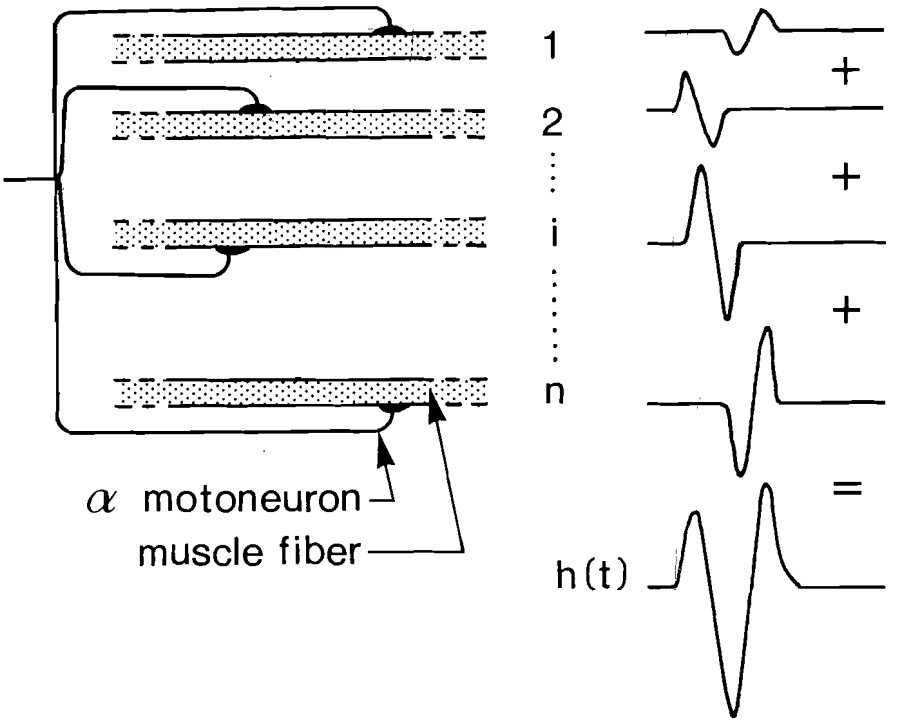
\includegraphics[width=0.6\linewidth]{./img/MUAP_oneMU.png}
\caption{Soma de potenciais de ação das \emph{n} fibras de uma unidade motora, formando uma MUAP \emph{h(t)}. Adaptado de BASMAJIAN e DE LUCA, 1985}
\label{fig:MUAP_comp}
\end{figure}
	
	Dependendo do método utilizado para aquisição de EMG, é comum a captura da contribuição de mais de uma unidade motora no mesmo canal. A influência de uma unidade motora no sinal adquirido depende principalmente da distância das fibras musculares ao ponto de aquisição (HAMMARBERG and STERNAD, 2002). A Figura \ref{fig:MUAP_soma} apresenta um exemplo com três unidades motoras, cujas MUAPs somadas compõem o sinal adquirido.
	
\begin{figure}
\centering
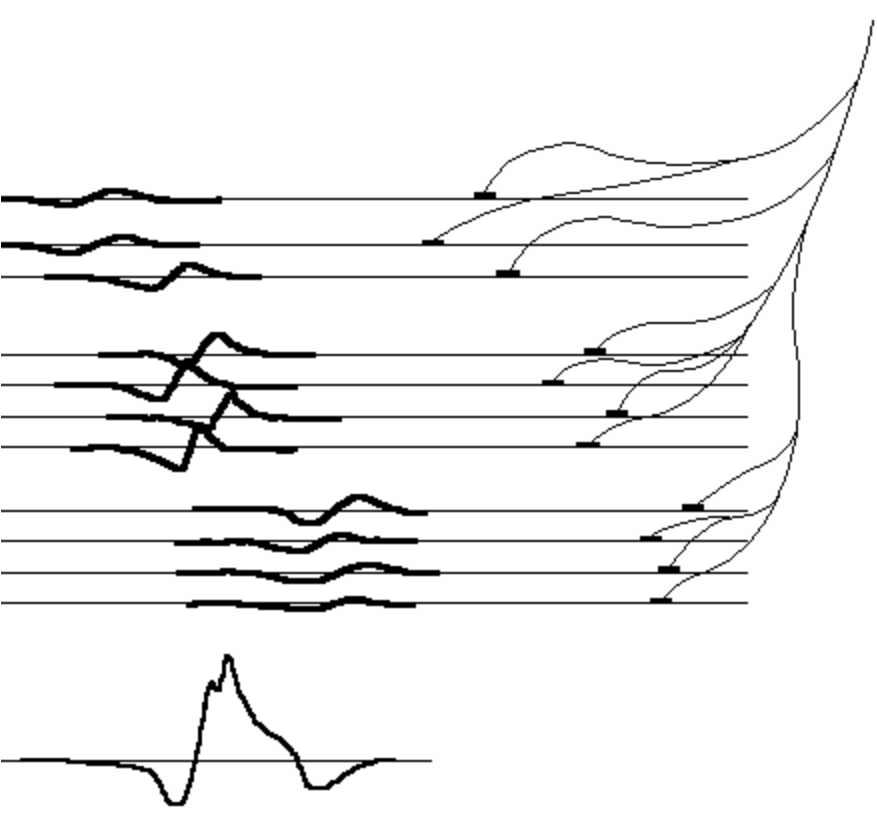
\includegraphics[width=0.6\linewidth]{./img/MUAP_soma.PNG}
\caption{Os sinais de MUAP correspondentes a três diferentes unidades motoras somam-se para formar o sinal adquirido por um canal de EMG. Adaptado de HAMMARBERG and STERNAD, 2002}
\label{fig:MUAP_soma}
\end{figure}
	
	Sinais de EMG de longa duração são constituídos por sequências temporais de MUAPs, também conhecidas como MUAPTs (\emph{MUAP Trains}). A Figura \ref{fig:MUAP_trains} exemplifica MUAPTs de diferentes MUs que somam-se para formar um sinal de EMG de longa duração.
	
\begin{figure}
\centering
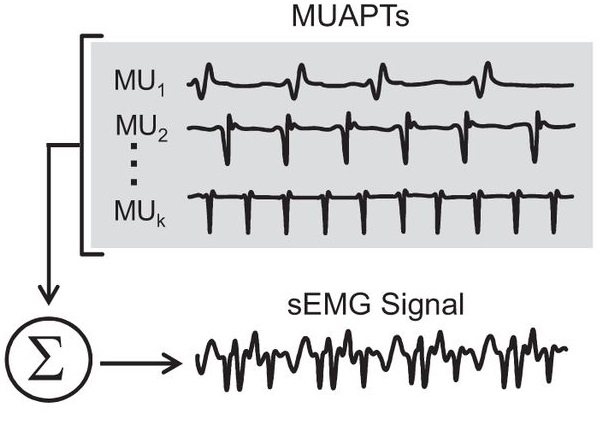
\includegraphics[width=0.6\linewidth]{./img/MUAP_trains.jpg}
\caption{MUAPTs de diferentes MUs somam-se para compor o sinal adquirido por um canal de EMG. Adaptado de KLINE and DE LUCA, 2014}
\label{fig:MUAP_trains}
\end{figure}

% ---
\section{Métodos de Segmentação}
% ---

	Esta seção descreve os métodos de segmentação originais que foram utilizados para basear os métodos implementados neste estudo. Nota-se que nomes utilizados para variáveis e constantes (e.g. `$r$', `$T$', etc.) foram determinados pelo autor deste estudo, não necessariamente sendo estes utilizados nos métodos originais.
	
\subsection{Método 1 (MTD1) - método iterativo para detecção de centros de segmentos de comprimento constante}

	Este é o método iterativo de segmentação utilizado em (CHAUVET et al, 2001). As variáveis e constantes da Tabela \ref{tab:mtd1params} serão utilizados para descrever este método.
	
\begin{table}[htb]
\IBGEtab{%
	\caption{Parâmetros utilizados para definir MTD1}%
	\label{tab:mtd1params}
}{%
	\begin{tabular}{ccc}
	\toprule
	Nome & Descrição \\
	\midrule \midrule
	$x$ & Sinal a ser segmentado \\
	$L$ & Comprimento total do sinal a ser segmentado \\
	\midrule
	$l$ & Comprimento desejado para segmentos \\
	\midrule
	$T_k$ & Valor de \emph{threshold} para a iteração $k$ \\
	\midrule 
	$q$ & Fração de $T_{k-1}$ para determinação de $T_k$ \\
	\midrule 
	$N_{k}$ & Número total de candidatos para centros de segmentos identificados na iteração $k$ \\
	\midrule 
	$r_k$ & Razão entre número de candidatos identificados na iteração $k$ e o comprimento total do sinal \\
	\midrule 
	$r_{target}$ & Razão mínima esperada para $r_k$, utilizada para determinar o final do método \\
	\bottomrule
\end{tabular}%
}{%
	\fonte{Do autor.}%
}
\end{table}
	
	Inicialmente, determina-se o valor de \emph{threshold} $T_0$ equivalente ao máximo absoluto do sinal a ser segmentado $x$ (equação \ref{eq:mtd1t0}). O valor $T_k$ é atualizado em cada iteração $k$ como sendo uma fração $q$ de $T_{k-1}$ (equação \ref{eq:mtd1tk}).
	
\begin{equation}
\label{eq:mtd1t0}
  T_0 = max(x)
\end{equation}

\begin{equation}
\label{eq:mtd1tk}
  T_k = q \times T_{k-1}
\end{equation}

	Pontos do sinal acima do valor de $T_k$ são possíveis candidatos para centros de segmentos. Caso exista mais de um possível candidato em uma vizinhança bilateral de $l$ amostras do sinal, apenas o ponto de maior amplitude nesta vizinhança é considerado.
	
	Para determinar o final do método, avalia-se a razão $r_k$ entre a quantidade identificada de candidatos $N_{k}$ e o comprimento total do sinal $L$ (equação \ref{eq:mtd1rk}). Caso $r_k$ seja menor que um valor predeterminado $r_{target}$, calcula-se $T_{k+1}$ para realização da próxima iteração (equação \ref{eq:mtd1tk}). Caso $r_k$ seja maior ou igual ao valor predeterminado $r_{target}$, encerra-se o método e os segmentos são tomados como janelas de sinal de comprimento $l$, centradas nos candidatos identificados na última iteração.
	
\begin{equation}
\label{eq:mtd1rk}
  r_k = \frac{N_{k}}{L} 
\end{equation}
	
	A Figura \ref{fig:mtd1flux} apresenta um fluxograma para as iterações do MTD1.
	
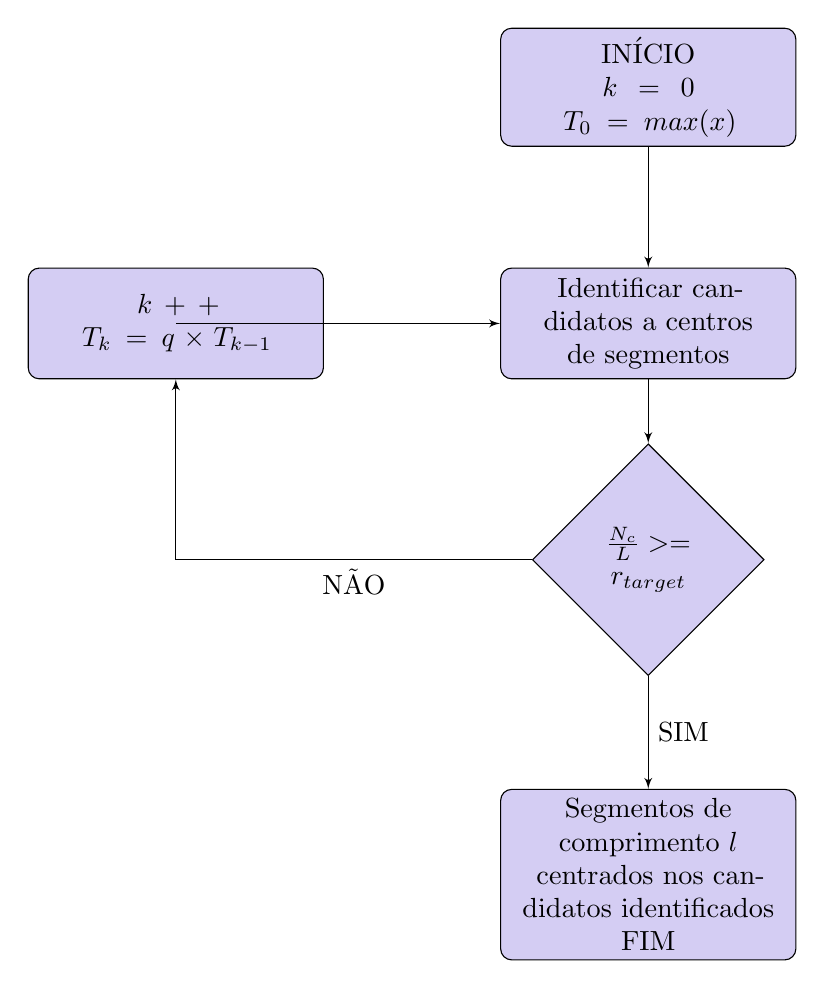
\begin{tikzpicture}[node distance = 2cm, auto]
    % Place nodes
    \node [block] (init) {INÍCIO\\$k = 0$\\$T_0 = max(x)$};
    \node [block, below of=init, node distance=3cm] (identify) {Identificar candidatos a centros de segmentos};
    \node [decision, below of=identify] (decide) {$\frac{N_c}{L} >= r_{target}$};
	\node [block, left of=identify, node distance=6cm] (update) {$k++$\\$T_k = q \times T_{k-1}$};
    \node [block, below of=decide, node distance=4cm] (stop) {Segmentos de comprimento $l$ centrados nos candidatos identificados \\ FIM};
    % Draw edges
    \path [line] (init) -- (identify);
    \path [line] (identify) -- (decide);
    \path [line] (decide) -| node [near start] {NÃO} (update);
    \path [line] (update) |- (identify);
    \path [line] (decide) -- node {SIM}(stop);
	
	\label{fig:mtd1flux}
\end{tikzpicture}
	
	Para ilustrar o MTD1, a Figura \ref{fig:mtd1example} apresenta uma implementação em trecho de sinal de EMG retirado da base de dados Ninapro, com fração $q$ de 90\% (isto é, $T_k = 0.9\times T_{k-1}$) e segmentos de comprimento $l$ de 400 amostras.
 
\begin{figure}
\centering
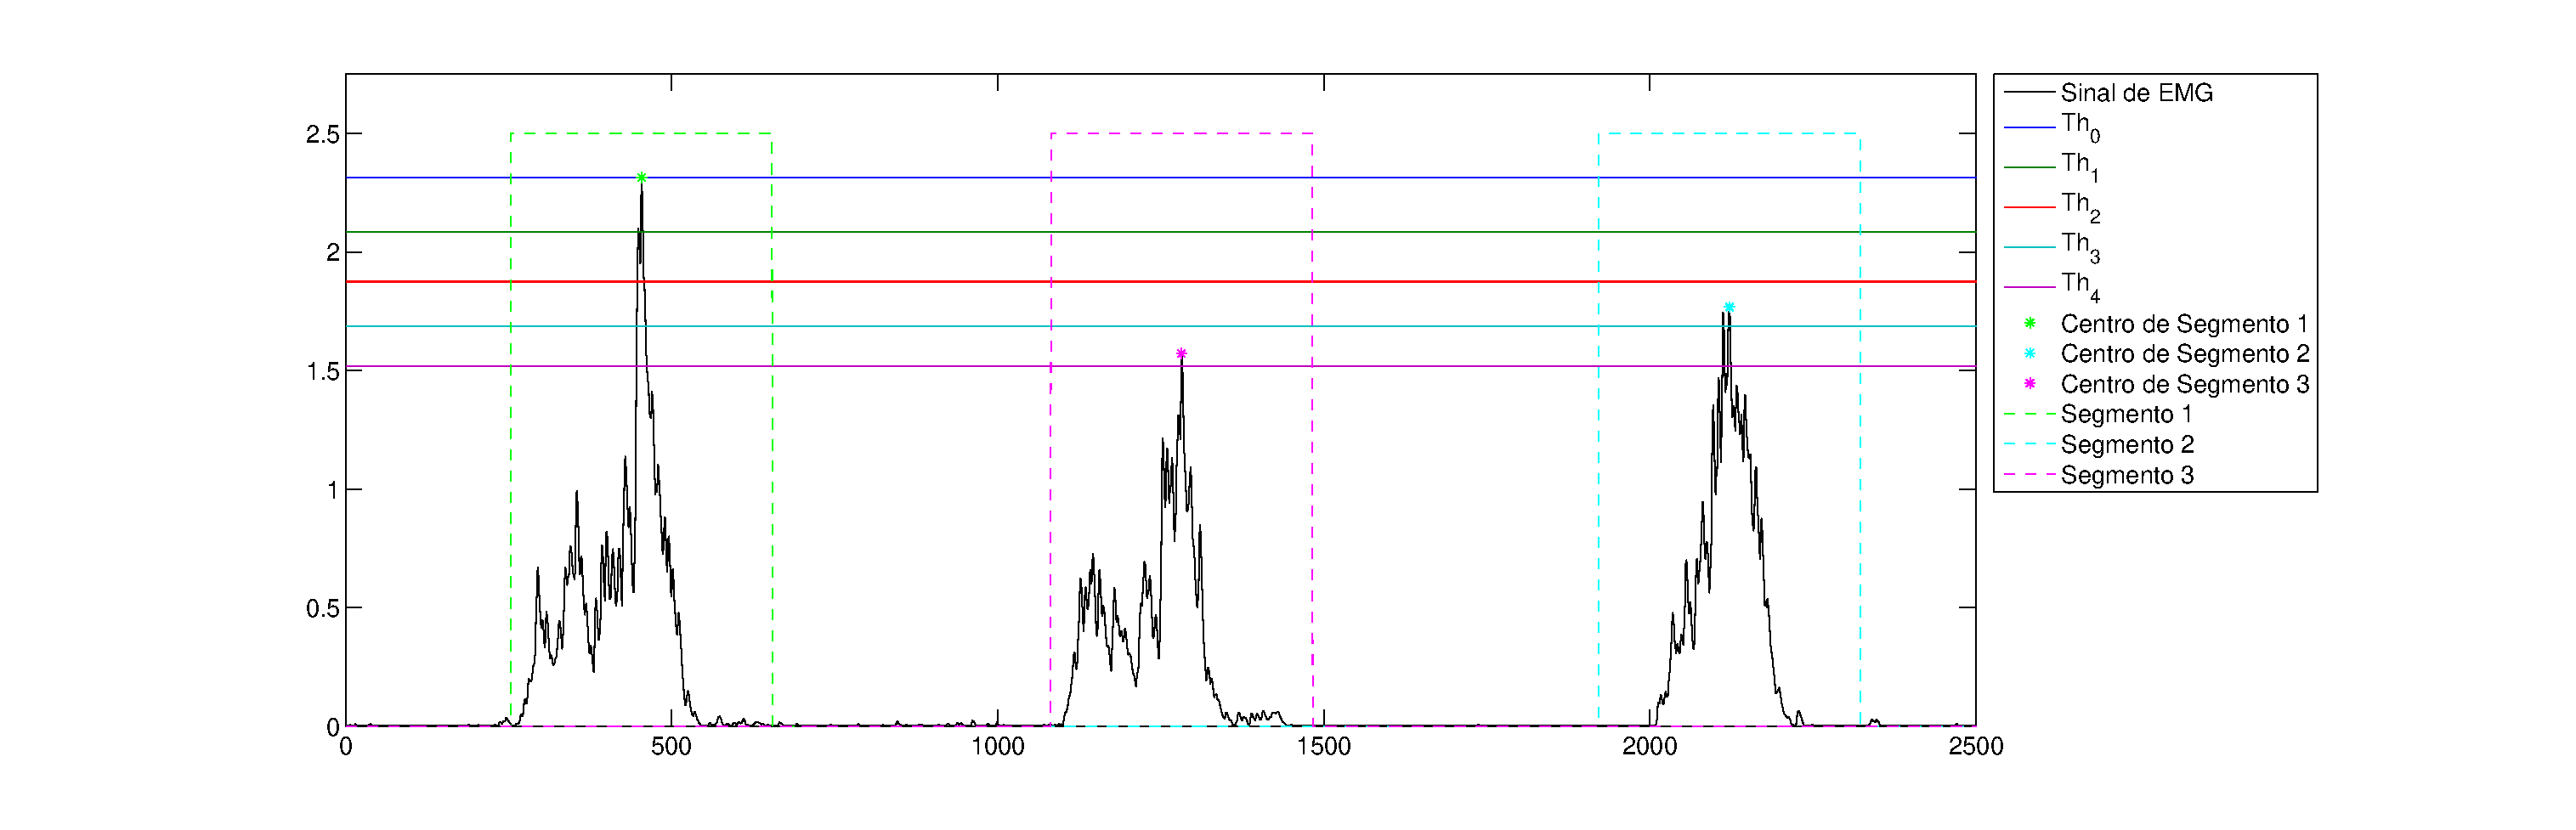
\includegraphics[width=\linewidth]{./img/mtd1example.eps}
\caption{Ilustração da implementação do MTD1, com $q = 0.9$ e $l = 400$. Do autor.}
\label{fig:mtd1example}
\end{figure}
 
\subsection{Método 2: detecção de picos de sinal e janelamento constante em torno dos picos}

	Este método é inspirado nos métodos utilizados nos trabalhos de (KATSIS et al 2003, 2006 e 2007). Primeiramente, detectam-se os picos de sinal acima de um determinado \emph{threshold} $T$ de amplitudes. Este \emph{threshold} $T$ deve ser obtido por relações entre a média, o comprimento e o valor máximo do sinal em questão. Na implementação original em (KATSIS et al, 2006), a relação utilizada para cálculo do \emph{threshold} $T$ é dada por \ref{eq:thKatsis}.

\begin{equation}
\label{eq:thKatsis}
  if\left(max(x_i) > \frac{30}{L}\sum_{i=1}^{L}|x_i|\right)
\end{equation}
\begin{center}
$then: T = \frac{5}{L}\sum_{i=1}^{L}|x_i|;$
$else: T = \frac{max(x_i)}{5}$
\end{center}

	Onde $L$ é o comprimento total do sinal de EMG $x$. Uma janela de comprimento constante (no caso de KATSIS 2006, utilizou-se 121 amostras) é centrada em cada elemento do sinal $x$ que seja superior ao \emph{threshold} T, e avalia-se se no interior da janela existe a ocorrência de valor de pico maior em amplitude que o pico original. Caso exista, este pico é o novo centro da janela e repete-se a verificação.

	Com este método, os sinais segmentados obtidos serão sempre de comprimento temporal constante e centrados em elementos correspondentes a extremos locais do sinal.

\subsection{Método 2: detecção de BEPs e EEPs}

	Este método é inspirado no método de segmentação utilizado em (PATTICHIS et al, 1995). Primeiramente, determina-se uma janela deslizante de comprimento $L$ associada a um \emph{threshold} de amplitudes $T$ (no trabalho original de PATTICHIS et al, 1995, o comprimento da janela era equivalente a 3 $ms$ e o \emph{threshold} era de $\pm$ 40 $\mu V$). Utilizando esta janela encontram-se os pontos do sinal chamados de BEP e EEP, ou simplesmente início e fim dos segmentos, de modo a atender as seguintes relações:

\begin{itemize}
\item{BEPs são pontos nos quais os elementos da janela de comprimento $L$ posicionada à esquerda permanecem menores que o \emph{threshold} $T$;}
\item{EEPs são pontos nos quais os elementos da janela de comprimento $L$ posicionada à direita permanecem menores que o \emph{threshold} $T$.}
\end{itemize}

	Para trechos consecutivos de elementos do sinal que atendem os critérios acima, o BEP escolhido deve ser o elemento mais à direita e o EEP deve ser o elemento mais à esquerda. BEPs e EEPs ocorrem de forma intercalada ao longo do sinal.
	
	Com este método, os sinais segmentados obtidos serão de comprimento variável, dependendo da duração do movimento realizado.
% ---
\section{Redes Neurais Artificias}
% ---

	TODO: REVISÃO SOBRE REDES NEURAIS

% ---
% Capitulo de Metodologia
% ---
\chapter{Metodologia Experimental}
% ---

\section{Aquisição de sinais}

	TODO: EXPLICAR COMO FORAM ADQUIRIDOS OS SINAIS DE (LOPES, 2014) E OS SINAIS DA BASE DE DADOS NINAPRO (ATZORI et al, 2012)

\section{Preprocessamento}

	TODO: RETIFICAÇÃO E FILTRAGEM DIGITAL DOS SINAIS

% ---
\section{Implementação dos Métodos de Segmentação}
% ---

	TODO: CÓDIGOS MATLAB

% ---
\section{Treinamento da Rede Neural Artificial}
% ---

	TODO: DESCRIÇÃO DOS VETORES DE PARÂMETROS UTILIZADOS
	TODO: IMPLEMENTAÇÃO DA REDE EM MATLAB

% ---
% Resultados
% ---
\chapter{Resultados e Discussões}
% ---


% ----------------------------------------------------------
% Finaliza a parte no bookmark do PDF
% para que se inicie o bookmark na raiz
% e adiciona espaço de parte no Sumário
% ----------------------------------------------------------
\phantompart

% ---
% Conclusão
% ---
\chapter{Conclusão}
% ---

% ----------------------------------------------------------
% ELEMENTOS PÓS-TEXTUAIS
% ----------------------------------------------------------
\postextual
% ----------------------------------------------------------

% ----------------------------------------------------------
% Referências bibliográficas
% ----------------------------------------------------------
\bibliography{abntex2-modelo-references}

\end{document}
